% options:
% thesis=B bachelor's thesis
% thesis=M master's thesis
% czech thesis in Czech language
% slovak thesis in Slovak language
% english thesis in English language
% hidelinks remove colour boxes around hyperlinks

\documentclass[thesis=B,english]{FITthesis}[2012/06/26]

\usepackage[utf8]{inputenc} % LaTeX source encoded as UTF-8

\usepackage{graphicx} %graphics files inclusion
\usepackage{amsmath} %advanced maths
\DeclareMathOperator*{\argmax}{argmax} % thin space, limits underneath in displays
% \usepackage{amssymb} %additional math symbols

\usepackage{dirtree} %directory tree visualisation

\usepackage{listings} %source code visualisation
\usepackage{xcolor}
\definecolor{dkgreen}{rgb}{0,0.6,0}
\definecolor{gray}{rgb}{0.5,0.5,0.5}
\definecolor{mauve}{rgb}{0.58,0,0.82}
\lstdefinestyle{myScalastyle}{
	frame=tb,
	language=scala,
	aboveskip=3mm,
	belowskip=3mm,
	showstringspaces=false,
	columns=flexible,
	basicstyle={\small\ttfamily},
	numbers=none,
	numberstyle=\tiny\color{gray},
	keywordstyle=\color{blue},
	commentstyle=\color{dkgreen},
	stringstyle=\color{mauve},
	frame=single,
	breaklines=true,
	breakatwhitespace=true,
	tabsize=3,
}

% % list of acronyms
% \usepackage[acronym,nonumberlist,toc,numberedsection=autolabel]{glossaries}
% \iflanguage{czech}{\renewcommand*{\acronymname}{Seznam pou{\v z}it{\' y}ch zkratek}}{}
% \makeglossaries

%\newcommand{\tg}{\mathop{\mathrm{tg}}} %cesky tangens
%\newcommand{\cotg}{\mathop{\mathrm{cotg}}} %cesky cotangens

% % % % % % % % % % % % % % % % % % % % % % % % % % % % % % 
% ODTUD DAL VSE ZMENTE
% % % % % % % % % % % % % % % % % % % % % % % % % % % % % % 

\department{Katedra teoretické informatiky}
\title{Paralelní implementace dynamického naivního Bayesovského klasifikátoru}
\authorGN{Pavel} %(křestní) jméno (jména) autora
\authorFN{Lučivňák} %příjmení autora
\authorWithDegrees{Pavel Lučivňák} %jméno autora včetně současných akademických titulů
\author{Pavel Lučivňák} %jméno autora bez akademických titulů
\supervisor{Ing. Tomáš Šabata}
\acknowledgements{Access to computing and storage facilities owned by parties and projects contributing to the National Grid Infrastructure MetaCentrum provided under the programme "Projects of Large Research, Development, and Innovations Infrastructures" (CESNET LM2015042), is greatly appreciated.}
\abstractCS{Dynamický naivní Bayesovský klasifikátor (DNBC) nachází využití v mnoha oblastech, například při rozpoznávání hlasu, písma, nebo při předpovídání počasí. DNBC je rozšířením skrytého Markovského modelu tím, že podporuje více pozorovaných proměnných. Předpokládá se, že tyto proměnné jsou vzájemně statisticky nezávislé. Tento předpoklad značně zjednodušuje výpočty a nedochází tak k jevu, který je znamý jako \textit{prokletí dimenzionatily}. Klasifikátor byl naimplementován v programovacím jazyce Scala, nad platformou Apache Spark. Tato implementace využívá dostupných výpočetních zdrojů, kde práce je rozdělena na více procesorů. Díky paralelizaci se mi podařilo zkrátit čas potřebný pro učení na polovinu (oproti sekvenční verzi). Demonstroval jsem, že zrychlení lze dosáhnout nejenom vyšším počtem jader, ale i vyšším počtem strojů.}
\abstractEN{Dynamic naive Bayesian networks (DNBC) have many applications, such as in speech recognition, handwriting recognition or weather prediction. DNBC extends a hidden Markov model by supporting multiple observed variables. It is assumed that these variables are mutually statistically independent. This assumption greatly simplifies computations and a phenomenon called \textit{curse of dimensionality} does not occur. I have implemented the classifier in Scala language on top of Apache Spark. My implementation makes use of computational resources available, distributing work load across multiple CPUs. Thanks to parallelization, I have shorten the time needed for learning by half (in comparison to the sequential implementation). I have further demonstrated, that the speed up can be achieved not only by increasing the number of cores, but also by increasing the number of machines in a cluster.}
\placeForDeclarationOfAuthenticity{V~Praze}
\declarationOfAuthenticityOption{4} %volba Prohlášení (číslo 1-6)
\keywordsCS{dynamický naivní Bayesovský klasifikátor, skrytý Markovův model, metoda maximální věrohodnosti, Scala, Apache Spark}
\keywordsEN{dynamic naive Bayesian classifier, hidden Markov model, maximum likelihood estimation, Scala, Apache Spark}
\website{https://github.com/lucivpav/dnbc-scala} %volitelná URL práce, objeví se v tiráži - úplně odstraňte, nemáte-li URL práce

\begin{document}

% \newacronym{CVUT}{{\v C}VUT}{{\v C}esk{\' e} vysok{\' e} u{\v c}en{\' i} technick{\' e} v Praze}
% \newacronym{FIT}{FIT}{Fakulta informa{\v c}n{\' i}ch technologi{\' i}}

\begin{introduction}
Hidden Markov model (HMM) is a probabilistic model that is widely used in many fields, e.g. for speech recognition, handwriting recognition or weather prediction. The model considers a hidden random variable and an observed random variable. In case of speech recognition, the hidden variable would be an actual letter from the alphabet a person said. The observed variable could then be a tone pitch. To estimate the current letter of a word that the person said, the model takes into account the previously said letter and the current pitch level.

The model is first trained using labeled data\textemdash containing both hidden states and observed states.\footnote{This is true if using maximum likelihood estimation method for learning. In case of Baum-Welch algorithm, only observed states and list of possible hidden states are necessary.} Then an inference can be used to predict hidden states, knowing only observed states.

A limitation of HMM is that it only supports one observed random variable. In case of the speech recognition, there are more variables than just tone pitch that are relevant to letter estimation. One could increase the dimensionality of the observed variable. However, this would lead to a phenomenon called \textit{curse of dimensionality} that would result in model training to be intractable.

Dynamic naive Bayesian classifier (DNBC) addresses this issue by supporting multiple observed variables. To avoid the curse of dimensionality, the observed variables are assumed to be statistically independent with each other. Due to the fact that the observed variables are statistically independent, the model can be easily trained in the parallel fashion.

However, there are no existing DNBC libraries written in Scala language. Although there exists a library for Bayesian networks, which is a super set of DNBC, it does not support parallelization on top of Apache Spark. Since Bayesian networks are above the scope of this thesis, I have decided to implement DNBC by myself.

In the first chapter, I briefly cover mathematical background used in this thesis\textemdash namely Gaussian distribution and Gaussian mixture distribution. Then I discuss parameter estimation of probabilistic models. This will be useful for training of HMM and DNBC later on.

In the Analysis chapter, I introduce foundations of DNBC. First, a Markov chain is introduced together with hidden Markov model. Afterwards, Bayesian networks and its derivatives, naive Bayesian classifier and dynamic Bayesian networks are discussed. This gives us enough foundation for defining dynamic naive Bayesian classifier.

DNBC is analyzed in terms of three basic operations that can be performed on it\textemdash learning, inference and scoring. I also provide an example problem and discuss limitations of DNBC.

The chapter \ref{ch:implementation} describes implementation details and design decisions I made when creating a DNBC library. Finally, I show experimental results on randomly generated data sets. The experiments are focused on learning and testing time. Scalability is measured as well. In the end, I show how well DNBC performs in terms of the inference accuracy on realistic data sets.
\end{introduction}

\chapter{Mathematical background}

\section{Probability density function}

Probability density function (PDF) of a continuous random variable determines a likelihood that a given value occurs. Furthermore, \ref{eq:pdf_interval} gives a probability of value being in interval $[a,b]$.

\begin{equation} \label{eq:pdf_interval}
P(a \leq x \leq b) = \int_a^b \text{PDF}(x) dx
\end{equation}

To satisfy the property that $P(-\inf < x < \inf) = 1$, the following has to hold:

\begin{equation}
\int_{-\inf}^{\inf} \text{PDF}(x) dx = 1.
\end{equation}

\section{Gaussian distribution}

Gaussian (normal) distribution is defined by a probability density function

\begin{equation} \label{eq:gaussian_pdf}
\text{PDF}_{\mathcal{N}(\mu,\sigma^2)}(x) = \frac{1}{\sqrt{2 \pi \sigma^2}}e^{-\frac{(x-\mu)^2}{2 \sigma^2}}.
\end{equation}

The distribution is defined by two parameters\textemdash mean $\mu$ and variance $\sigma^2$. Figure \ref{fig:gaussian} provides a visualization of the probability density function.

\begin{figure}
	\centering
 	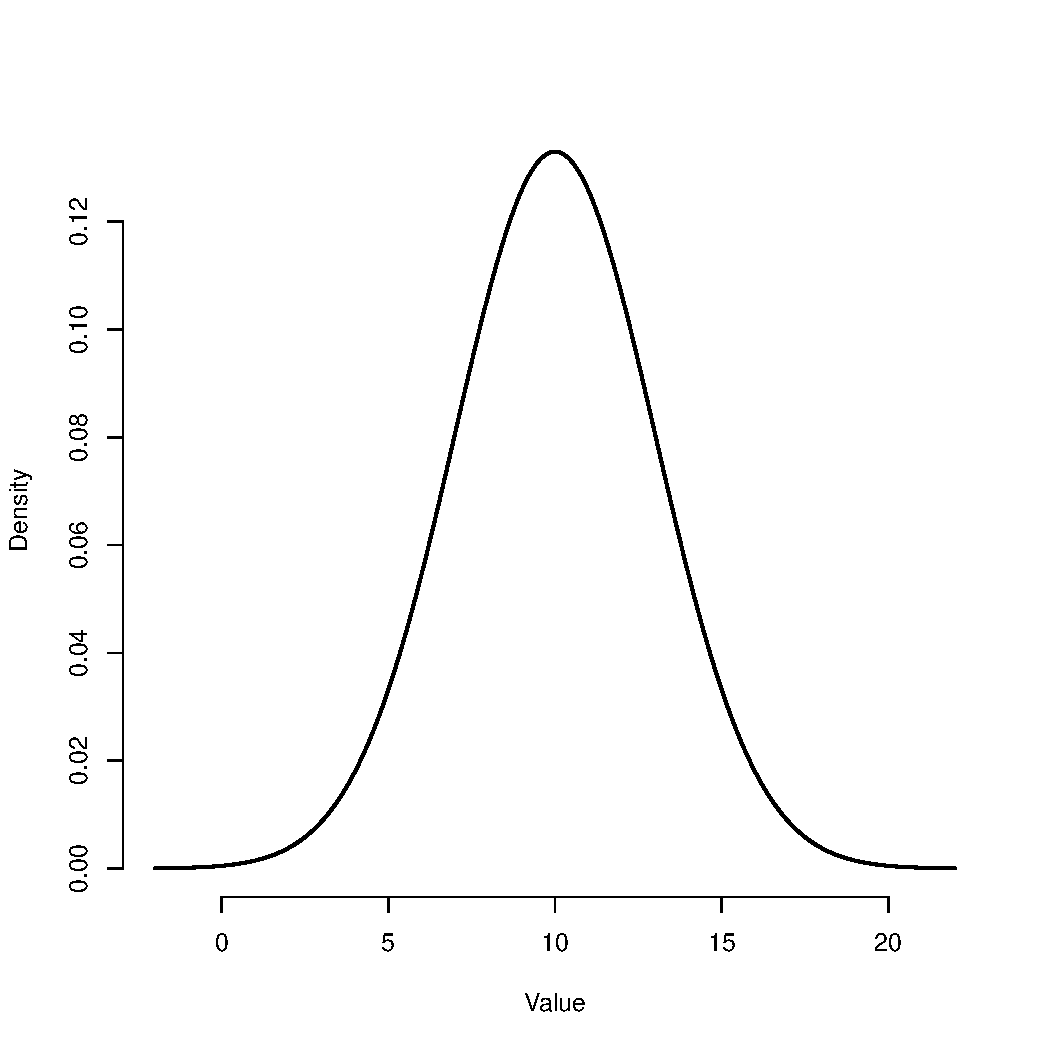
\includegraphics[width=0.7\textwidth]{gaussian}
 	\caption{Visualization of Gaussian PDF with parameters $\mu=10$ and $\sigma^2=3^2$.}
 	\label{fig:gaussian}
\end{figure}

Normal distribution is one of the most widespread distribution found in nature \cite{gaussian-distribution-widespread}. Imagine $n$ independent, identically distributed (i.i.d.) random variables. For large $n > 30$, both sum and average of the variables converge to normal distribution. This phenomenon occurs because of the Central Limit Theorem. See book \textit{Introduction to Probability} \cite{clt-proof} for a proof.

\section{Gaussian mixture distribution}

Gaussian mixture distribution is a weighted sum of multiple components that follow normal distribution. The PDF is given by \ref{eq:gaussian_mixture_pdf}, where $n$ is number of components.

\begin{equation} \label{eq:gaussian_mixture_pdf}
\text{PDF}_{\mathcal{N}^*(\theta)}(x) = \sum_{i=1}^n w_i \text{PDF}_{\mathcal{N}(\mu_i,\sigma^2_i)}(x),
\end{equation}

where $w_i$ is a weight of particular component. The following conditions have to hold:

\begin{equation}
w_i \geq 0, 1 \leq i \leq n,
\end{equation}

\begin{equation}
\sum_{i=1}^n w_i = 1.
\end{equation}

\begin{figure}
	\centering
 	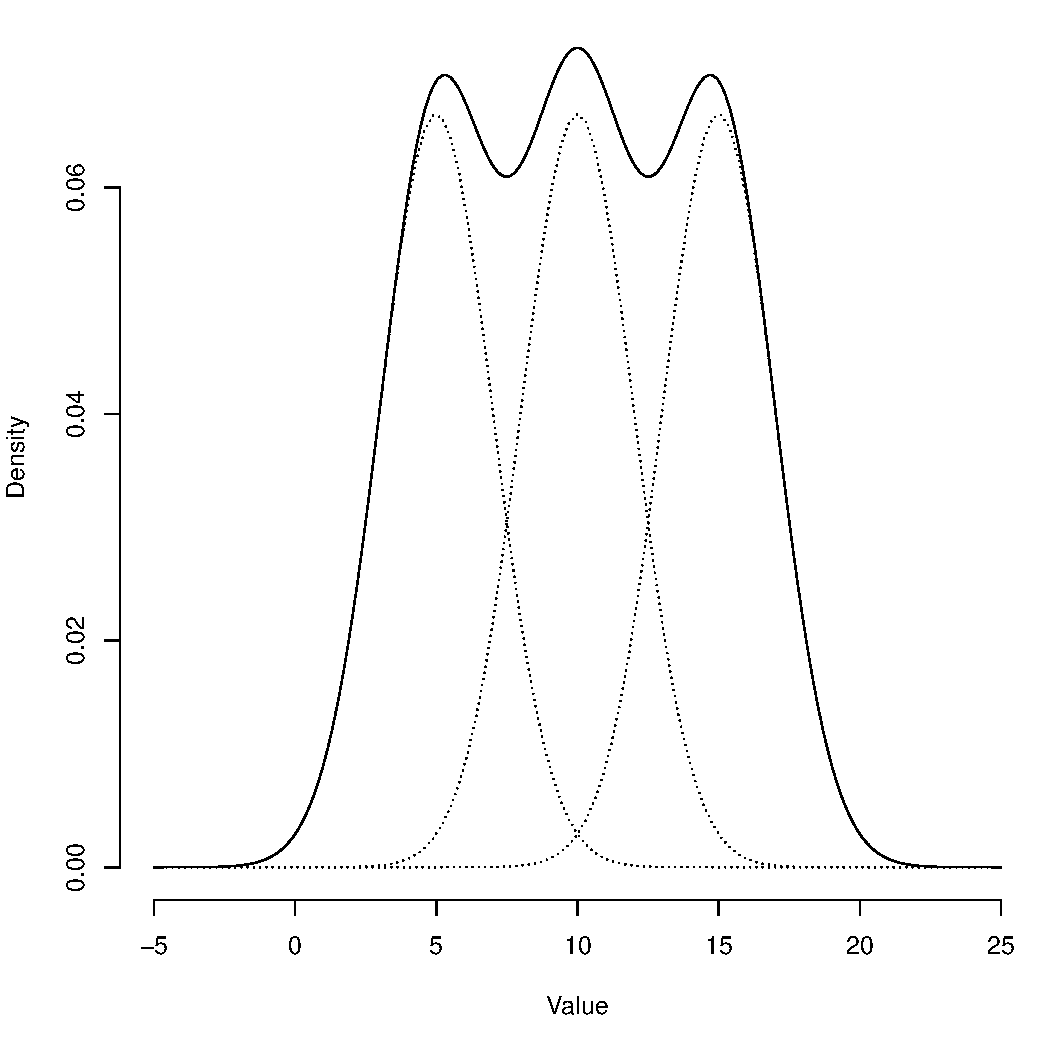
\includegraphics[width=0.7\textwidth]{gaussian_mixture}
 	\caption{Visualization of a mixture with three components with parameters $\mu_1=5, \mu_2=10, \mu_3=15$ and $\sigma_{1,2,3}^2=2^2$. Weights are $w_{1,2,3} = \frac{1}{3}$. Author: Smason79 \cite{gaussian-mixture}.}
 	\label{fig:gaussian_mixture}
\end{figure}

\chapter{Parameter estimation}
\label{parameter-estimation-chapter}
In context of this chapter, the goal of parameter estimation is to estimate parameters of a probability distribution in a way that describes given data the best.

\section{Maximum likelihood estimation}
Maximum likelihood estimation (MLE) is a technique for finding parameters of a probabilistic distribution that best describe a random variable. The method aims to maximize the likelihood of all the learning data.

Formally $\argmax_{\theta \in \Theta} \prod_{j=1}^{M} L(x_j, \theta)$, where:

\begin{itemize}

\item $M$ is number of data points,
\item $X = \{x_1, x_2, \dots, x_M\}$ is a learning set of data points,
\item \emph{L} is a likelihood function (defined further),
\item $\theta$ describes model parameters,
\item $\Theta$ is a set of all model parameters.

\end{itemize}

\section{Discrete distribution}

Here I present a straightforward way of defining the likelihood function in case of discrete random variables. $L(x,\theta) = x_{cnt} / M$, where $x_{cnt}$ is the number of times $x \in X$ occurs in learning data. Since the likelihood function does not depend on parameter $\theta$, there is no expression to optimize.

There is a reason I did not choose any standard discrete probability distribution to define $L$. The random variable does not have to be \textbf Z, nor \textbf N. In fact it can be any abstract object, such as an animal. A type, where comparison between two objects doesn't make sense. Therefore, it wouldn't make sense to assign non-zero probability to values that are not specified in learning phase.

As an example, consider the following data: \{dog, bird, dog, cat, bird, dog\}. Figure \ref{fig:discrete_mle_prob} shows a likelihood function $L$ associated with the data.

% TODO: consider two figures side by side
\begin{figure}
	\centering
 	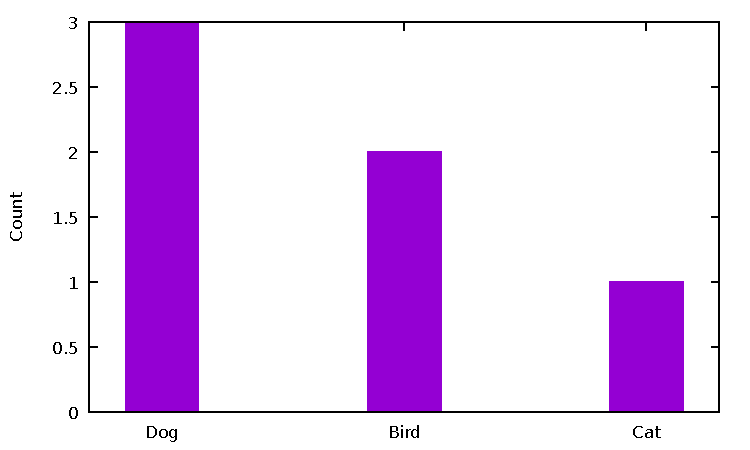
\includegraphics[width=0.7\textwidth]{discrete_mle_hist}
 	\caption{Frequency of data in a discrete data set.}
 	\label{fig:discrete_mle_hist}
\end{figure}

\begin{figure}
	\centering
 	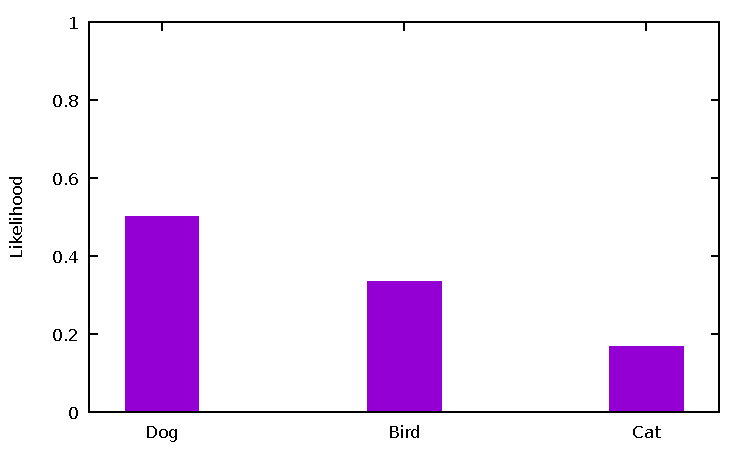
\includegraphics[width=0.7\textwidth]{discrete_mle_prob}
 	\caption{Likelihood function $L$ of data in the discrete data set. Likelihood is zero at undefined states.}
 	\label{fig:discrete_mle_prob}
\end{figure}

\section{Gaussian distribution}

\begin{figure}
	\centering
 	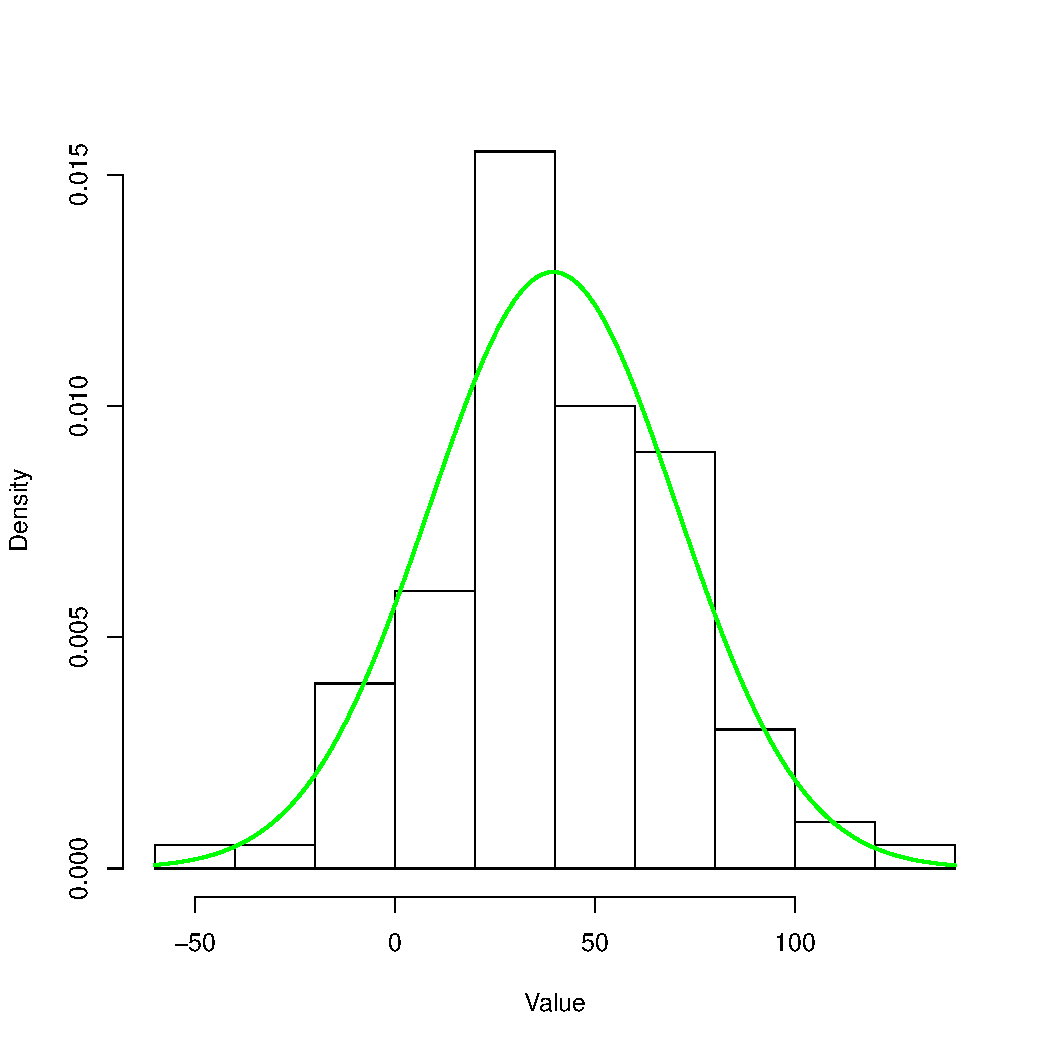
\includegraphics[width=0.7\textwidth]{normal_mle}
 	\caption{Histogram of randomly generated data from normal distribution $\mathcal{N}(40,32^2)$. The green curve is a plot of normal distribution with the maximum likelihood estimate of $\theta$ parameters.}
 	\label{fig:normal_mle}
\end{figure}

The normal distribution is defined by $\theta = \{\mu, \sigma^2\}$. In MLE, the goal is to find parameter $\theta \in \Theta$, such that the product in \ref{eq:gaussian_mle_prod} is maximized.

\begin{equation} \label{eq:gaussian_mle_prod}
\prod_{j=1}^{M} L(x_j, \theta)
\end{equation}

In the case of Gaussian distribution, the likelihood function $L$ is defined by

\begin{equation*}
L(x, \theta) = \frac{1}{\sqrt{2 \pi \sigma^2}}e^{-\frac{(x-\mu)^2}{2 \sigma^2}},
\end{equation*}

\medskip
where $x \in X$. Taking derivative of \ref{eq:gaussian_mle_prod} with respect to $\mu$ equal to 0 yields

\begin{equation*}
\sum_{j=1}^{M}{x_j - M \mu} = 0.
\end{equation*}

\bigskip
Maximum likelihood estimate of $\mu$ is therefore

\begin{equation*}
\mu_{\text{est}} = \overline X_M.
\end{equation*}

\medskip
Derivative of \ref{eq:gaussian_mle_prod} with respect to $\sigma^2$ equal to zero results in MLE of $\sigma^2$ to be

\begin{equation*}
\sigma^2_{\text{est}} = \frac{1}{M} \sum_{j=1}^{M} {(x_j-\overline X_M)^2}.
\end{equation*}

Figure \ref{fig:normal_mle} shows an example of MLE on a normally distributed random variable.

\section{Gaussian mixture distribution}

\begin{figure}
	\centering
 	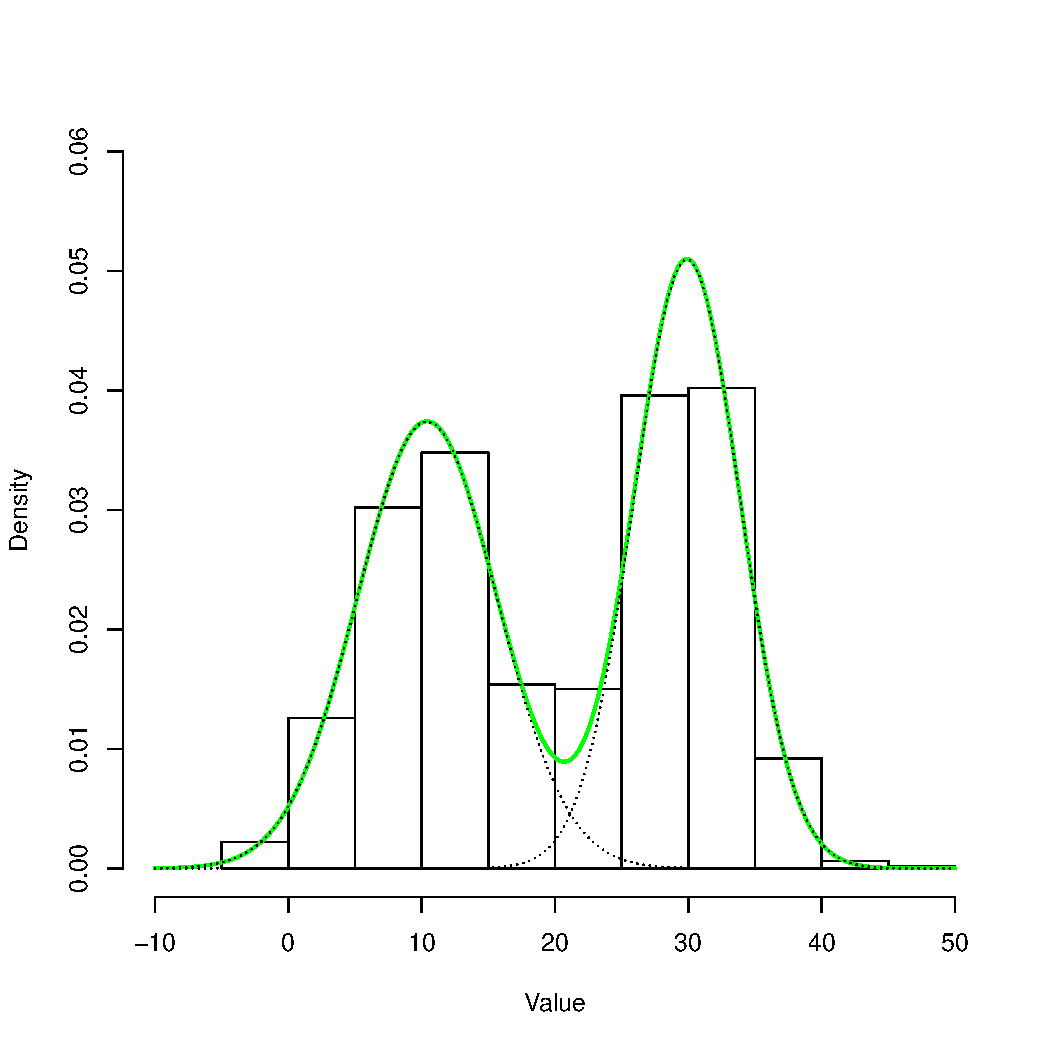
\includegraphics[width=0.7\textwidth]{gaussian_mixture_estimate}
 	\caption{Histogram of randomly generated data from two normal distributions $\mathcal{N}(10,5^2)$ and $\mathcal{N}(30,4^2)$. The green curve is the best estimate, found using EM algorithm, of underlying normal mixture distribution. Dotted curves are estimates of individual Gaussian mixture components.}
 	\label{fig:gaussian_mixture_est}
\end{figure}

Given the number of components $K$ components, there are component parameters $\theta_1, \theta_2, \dots, \theta_K$ and weights $w_1, w_2, \dots, w_K$ to estimate. In this section, I provide a description of expectation-maximization algorithm based on the lecture notes by Padhraic Smyth \cite{gaussian-mixture-em}. This algorithm provides an estimate of the aforementioned parameters.

Let's define a membership weight $w_{jk}$, of data point $x_j$ in component $k$ as

\begin{equation*}
w_{jk} = \frac{\alpha_k \text{PDF}_{\mathcal{N}(\theta_k)}(x_j)}{\sum_{i=1}^K \alpha_i \text{PDF}_{\mathcal{N}(\theta_i)}(x_j)},
\end{equation*}

where $\alpha_k$ is a probability that a randomly selected $x_j$ was generated by the component $k$. $w_{jk}$ can be thought of as a level of certainty that $x_j$ was generated by the component $k$. $\sum_{k=1}^K w_{jk} = 1$ holds.

The likelihood of all data points given Gaussian mixture parameters is defined as

\begin{equation} \label{eq:gaussian_mixture_likelihood}
l = \sum_{j=1}^{M} \sum_{k=1}^{K} \alpha_k \text{PDF}_{\mathcal{N}(\theta_k)}(x_j).
\end{equation}

EM is an iterative algorithm, typically iterating until convergence is detected. Each iteration consists of two parts, an E-step and an M-step. In the E-step, weight $w_{jk}$ is computed for each data point $x_j$ and component $k$. Define $W_k = \sum_{j=1}^{M} w_{jk}$, the weight of all data points in component $k$. In the M-step, new model parameters are calculated as follows:

\begin{equation*}
\alpha_k^{\text{new}} = \frac{W_k}{M},
\end{equation*}

\begin{equation*}
\mu_k^{\text{new}} = \frac{\sum_{j=1}^M w_{jk} x_j}{W_k},
\end{equation*}

\begin{equation*}
{\sigma_k^{2}}^{\text{new}} = \frac{\sum_{j=1}^M w_{jk} (x_j-\mu_k^{\text{new}})^2}{W_k}.
\end{equation*}

Where $\mu_k^{\text{new}}$ resembles standard equation for estimating mean, and 
${\sigma_k^{2}}^{\text{new}}$ is similar to an equation for estimating variance. The differences are in weighting.

In the beginning of the algorithm, an initial guess of model parameters is necessary. This can be chosen randomly or through a heuristic.

Termination of the algorithm is determined by checking that the likelihood \ref{eq:gaussian_mixture_likelihood} of all data points hasn't improved enough in between iterations. In other words

\begin{equation*}
l_{\text{cur}} - l_{\text{prev}} < \text{tol}.
\end{equation*}

One issue with the EM algorithm is that it does not guarantee to find a global optimum.

\chapter{Analysis}

\section{Markov chain}

\subsection{Introduction}
Markov chain describes possible sequences of events in which a probability of being at a state at given time depends only on value of previous state. 

\subsection{Description}

Markov chain is defined by

\begin{itemize}
\item a set of states $S = \{S_1, S_2, \dots, S_N\}$,
\item a transition matrix $A \in \textbf R^{N \times N}$,
\item an initial probability vector $\pi \in \textbf R^N$.
\end{itemize}

Where $a_{ij}, 1 \leq i,j \leq N$ is a probability of transitioning from state $S_i$ into state $S_j$. $\pi_i$ is a probability that the initial state is $S_i$.

Suppose a sequence of states $y_1, y_2, \dots, y_T$, where $T \geq 2$. At time $t$, where $1 \leq t \leq T-1$, the transition probability $a_{ij}$ is defined as $P(y_{t+1}=S_j | y_t=S_i)$.

\subsection{Markov property}
Markov chain satisfies a Markov property. This property says that $P(y_{t+1}=S_i|y_1=s_1,y_2=s_2,\dots,y_t=s_t) = P(y_{t+1}=S_{i}|y_t=s_t)$. In other words, being at state $S_i$ at time $t+1$ only conditionally depends on being at state $s_t$ at time $t$. Further history doesn't influence the probability.

\subsection{Example}

\begin{figure}
	\centering
 	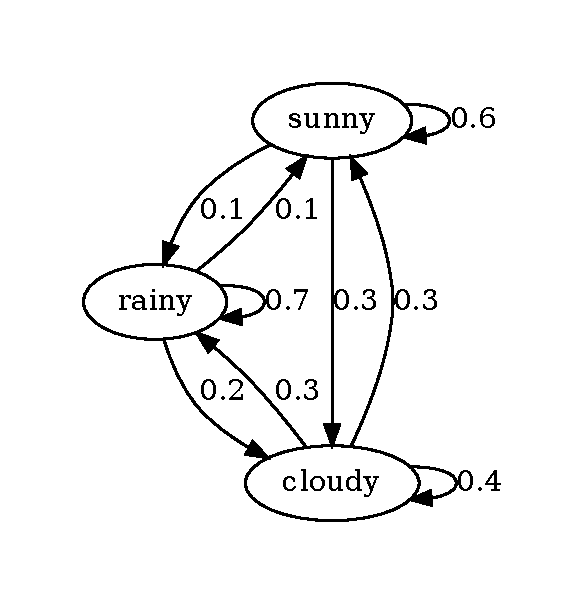
\includegraphics[width=0.7\textwidth]{mc}
 	\caption{Visualization of a Markov chain with three states.}
 	\label{fig:mc}
\end{figure}

As an example, consider a Markov chain (MC) with three states: $S_1 = \text{sunny}$, $S_2 = \text{rainy}$ and $S_3 = \text{cloudy}$. This MC models how weather changes on every day. Suppose the following transition matrix:

\begin{equation*}
A =
\begin{bmatrix}
	0.6	& 0.1 & 0.3 \\
	0.1 & 0.7 & 0.2 \\
	0.3 & 0.3 & 0.4
\end{bmatrix}.
\end{equation*}

The transition matrix is readable for a human. For example, if the weather is sunny, tomorrow will be most likely sunny as well. With probability 0.3, it will be cloudy. Rainy weather is very unlikely tomorrow. Consider the following initial probability vector:

\begin{equation*}
\pi = \begin{bmatrix} 0.3 \\ 0.2 \\ 0.5 \end{bmatrix}.
\end{equation*}

As it can be seen, the most likely weather on first day of measurement is cloudy.

\subsection{Limitations}

The previous example only takes into account the weather at time $t$ to predict the weather at time $t+1$. In the reality, there are multiple factors that influence what the weather will be like. According to the example, if a weather is sunny now, it is relatively unlikely it will start raining. If we, however, take into account a humidity, we can improve the prediction. If we know that the humidity is high, even though it was sunny, we can predict it started raining. Hidden Markov model addresses this issue.

\section{Hidden Markov model}

\subsection{Introduction}

Hidden Markov model (HMM) is an extension of Markov chain. The states are now called hidden states and every hidden state has an associated observed state.

\subsection{Description}

HMM is defined by (based on paper by L. Rabiner \cite{hmm-lawrence}):
\begin{itemize}

\item a set of hidden states $S = \{S_1, S_2, \dots, S_N\}$,
\item a set of observed symbols $X$,
\item a transition matrix $A \in \textbf R^{N \times N}$,
\item an observation probability functions $B = \{b_1(o), b_2(o), \dots, b_N(o)\}$,
\item an initial probability vector $\pi \in \textbf R^N$.

\end{itemize}

The values of the $X$ can be either discrete or continuous. The values of $S$ are assumed to be discrete. The observation probability function $b_i(o)$ describes a probability $P(x_t = o | y_t = S_i)$, where $o \in X$. This probability function is also called an emission function.

Imagine a walk through a HMM graph (see figure \ref{fig:hmm_graph} for an example graph). At each time point $t$, there is a hidden state $y_t$ and an observed symbol $x_t$. A value of the observed symbol conditionally depends on a value of the hidden state. The dependency is described by emission function $b_i(o)$.

If $t \neq 1$ and $T > 1$, there is a hidden state $y_t$ that conditionally depends on a value of previous hidden state $y_{t-1}$. The dependency is described by the transition $a_{ij}$. If $t = 1$, there is a hidden state $y_1$ that conditionally depends on the initial transition $\pi_i$.

\begin{figure}
	\centering
 	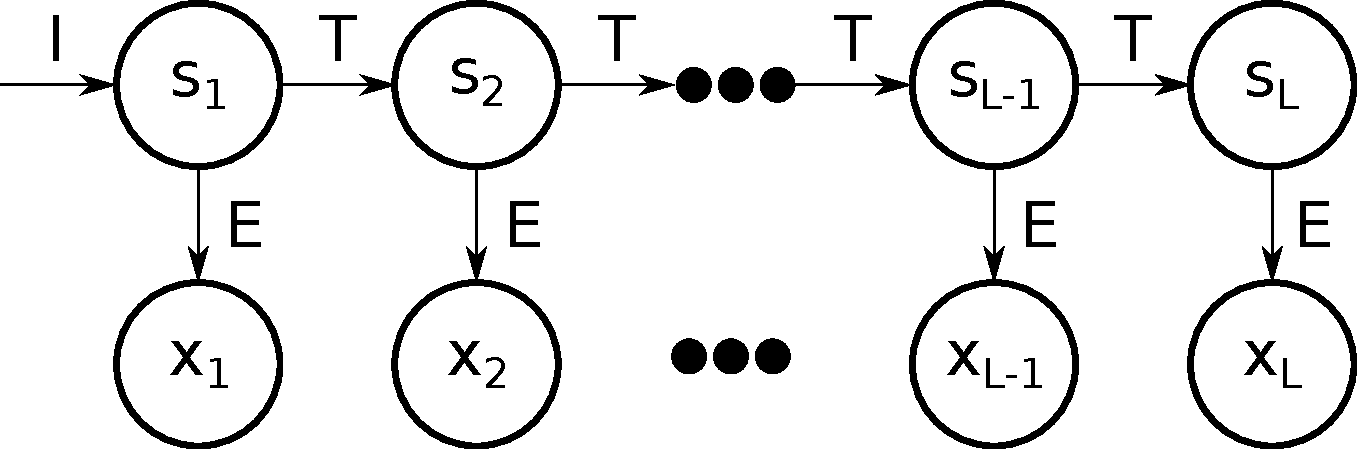
\includegraphics[width=0.7\textwidth]{hmm}
 	\caption{Visualization of a walk through a hidden Markov model. At each time point, there is a hidden state $y_t$ and an observed symbol $x_t$.}
 	\label{fig:hmm}
\end{figure}

\subsection{Operations}

There are three common operations that can be performed on HMM\textemdash learning, inference and scoring.

Learning is used to estimate the model parameters $\{\pi, A, B\} = \lambda$. It is desired to estimate the parameters such that $\prod_{j=1}^{M} P(\textbf x_j | \lambda )$ is maximized. Where $M \in \textbf N$ is a number of sequences used in learning. $\textbf x_j$ is a \emph{j}-th sequence of observed symbols. In other words, it is desired to maximize the probability that given sequences of observed symbols were generated by the model.

Inference returns the most likely sequence of hidden states, given a sequence of observed symbols.

Given a sequence of observed symbols $x_1, x_2, \dots, x_T$, what is the probability that the sequence was generated by HMM with parameters $\lambda$? Scoring answers this question.

\subsection{Learning}

\paragraph{Initial transition function}

The initial probability vector $\pi$ can be viewed as a probability function $\pi_i$, assigning a probability to every hidden state $S_i \in S$. This is a function of discrete random variable that defines discrete probability distribution. As such, MLE technique (discussed in chapter \ref{parameter-estimation-chapter}) can be used to estimate the distribution parameters.

\paragraph{Transition function}

Every row of $A$ defines a probability function $a_{ij}$. These functions are called transition functions. The transition functions define discrete probability distributions. Parameters of every such distribution can be estimated using MLE.

\paragraph{Emission function}

The observation probability functions $b_i(o)$ are functions of either discrete or continuous random variable that takes on values in set of observed symbols $X$. For purposes of this thesis, it is assumed that continuous variables follow a Gaussian or Gaussian mixture distribution.

The functions $b_i(o)$ are also called emission functions (emissions). If values of the set of observed symbols $X$ are discrete, then the emissions define discrete distributions and the parameters can be estimated through MLE. If the values of $X$ are continuous, then the emissions define continuous probability distributions. As discussed earlier, parameters of Gaussian distribution can be estimated using MLE. Parameters of Gaussian mixture distribution can be estimated through EM algorithm.

\paragraph{Baum-Welch training}

Baum-Welch training is an alternative learning algorithm that is not based on the MLE approach. It will not be covered in this thesis, but its existence should be noted in case you are a curious reader \cite{hmm-lawrence}.

\subsection{Inference}

Given a sequence of observed symbols, what is the most likely associated sequence of hidden states? Viterbi algorithm answers this question. Let's define $\alpha_t(i)$ to be the maximum probability of sequence of hidden states and observed symbols up to time point $t$:

\begin{equation} \label{eq:hmm_viterbi_a}
\alpha_t(i) = max_{y_1,y_2,\dots,y_{t-1}} P(y_1,y_2,\dots,y_{t-1},y_t = S_i,x_1,x_2,\dots,x_t | \lambda),
\end{equation}

where $\lambda$ are parameters of HMM model.

\paragraph{Initialization}

At time point $t=1$, the probability of being at hidden state $S_i$ is simply the initial probability of being at that state and a probability of being at observed state $x_1$ given hidden state $S_i$. In other words:

\begin{equation*}
\alpha_1(i) = \pi_i b_i(x_1).
\end{equation*}

\paragraph{Recursion}
Taking into account the structure of HMM, the equation \ref{eq:hmm_viterbi_a} can be rewritten recursively as

\begin{equation} \label{eq:hmm_viterbi_a_rec}
\alpha_t(j) = [\max_i \alpha_{t-1}(i)a_{ij}] b_j(x_t).
\end{equation}
Hidden state at particular time point $t$ is determined by

\begin{equation*}
s_t = S_{\argmax_i \alpha_{t}(i)}.
\end{equation*}

\paragraph{Complexity}

At each time point $t$ and hidden state index $j$, the equation \ref{eq:hmm_viterbi_a_rec} loops through every hidden state index $i$. There are $N$ hidden states. In addition, the recursion continues for every time point $t$. There are $T$ time points. Thus, the overall complexity is
$N^2 T$.

\subsection{Scoring}

In previous section, I have defined $\alpha_t(i)$ to be a probability of a sequence of hidden states up to time point $t$, where $y_t = S_i$, and a sequence of observed symbols up to time point $t$, given model parameters.

In order to compute the probability that sequence of observed symbols was generated by the HMM (score), take a look how $\alpha_T(i)$ is defined:

\begin{equation*}
\alpha_T(i) = max_{y_1,y_2,\dots,y_{T-1}} P(y_1,y_2,\dots,y_{T-1},y_T = S_i,x_1,x_2,\dots,x_T | \lambda).
\end{equation*}
The score is then

\begin{equation*}
\sum_{i=1}^{N} \alpha_T(i).
\end{equation*}

\subsection{Example}

\begin{figure}
	\centering
 	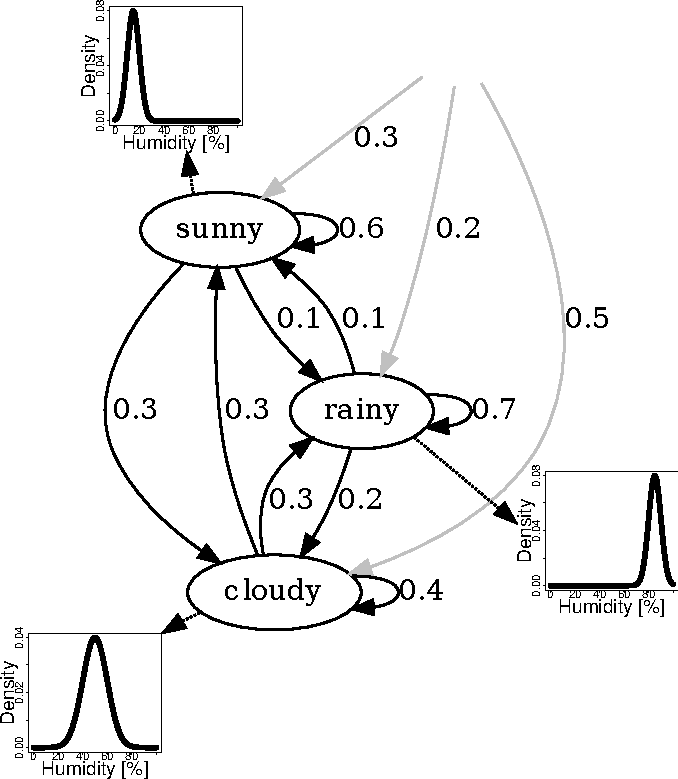
\includegraphics[width=0.7\textwidth]{hmm-graph}
 	\caption{Visualization of a hidden Markov model with three states and a continuous observed variable.}
 	\label{fig:hmm_graph}
\end{figure}

Suppose an extension of an example mentioned in Markov chain chapter. i.e. there are three hidden states of weather: $S_1 = \text{sunny}$, $S_2 = \text{rainy}$ and $S_3 = \text{cloudy}$. Let's introduce a continuous observed random variable describing humidity level. It is easy to imagine that on sunny day, the humidity will be typically lower than on a rainy day. This observable variable can help in predicting future weather. The example is depicted in figure \ref{fig:hmm_graph}.

\subsection{Limitations}
There is only one observed variable, which may not be sufficient for successful prediction in real-life applications. One could increase the dimensionality of the observed variable. That would, however, lead to a problem called \textit{curse of dimensionality}. As we would increase the dimensionality of observed variable, the learning time would increase greatly up to the point where it would no longer be tractable. More training data would be necessary too. Dynamic naive Bayesian classifier addresses this issue.

\section{Bayesian network}

Bayesian network is a probabilistic graphical model consisting of nodes and edges. The model is a directed acyclic graph (DAG). Every node describes a random variable which can be either discrete or continuous. Edges describe a conditional dependency among the nodes (variables).

As an example, consider a Bayesian network in figure \ref{fig:bn}. In the example, every node represents a discrete random variable with two possible states\textemdash\textit{true} and $false$. It can be interpreted that dehydration can cause red skin, but it can also influence presence of cancer. In addition, red skin may signal a lack of water intake, or the skin may be red because of cancer cells. Every node defines a conditional probability table (CPT) given nodes it depends on.

\begin{figure}
	\centering
 	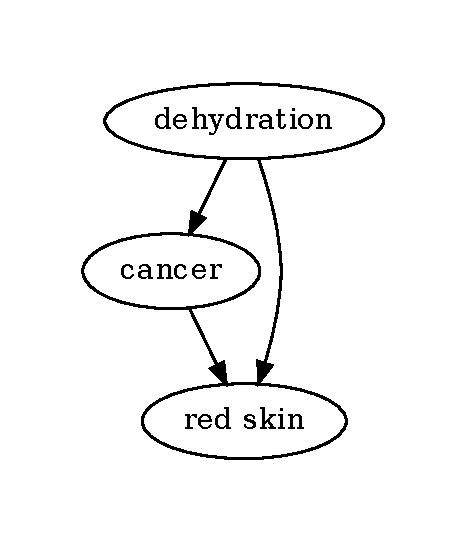
\includegraphics[width=0.7\textwidth]{bn}
 	\caption{Visualization of a Bayesian network with three states.}
 	\label{fig:bn}
\end{figure}

\begin{table}
\parbox{0.45\linewidth}{
\centering
\begin{tabular}{|c|c|}
\hline
\multicolumn{2}{|c|}{dehydration}  \\
\hline
true & false \\
\hline
0.1 & 0.9 \\
\hline
\end{tabular}
\caption{CPT for $dehydration$.}
}
\hfill
\parbox{0.45\linewidth}{
\centering
\begin{tabular}{|c||c|c|}
\hline
input & \multicolumn{2}{c|}{cancer} \\
\hline
dehydration & true & false \\
\hline
true & 0.1 & 0.9 \\
\hline
false & 0.01 & 0.99 \\
\hline
\end{tabular}
\caption{CPT for $cancer$.}
}
\centering
\begin{tabular}{|c|c||c|c|}
\hline
\multicolumn{2}{|c||}{input} & \multicolumn{2}{c|}{red skin} \\
\hline
cancer & dehydration & true & false \\
\hline
true & true & 0.4 & 0.6 \\
\hline
true & false & 0.3 & 0.7 \\
\hline
false & true & 0.4 & 0.6 \\
\hline
false & false & 0.1 & 0.9 \\
\hline
\end{tabular}
\caption{CPT for $red$ $skin$.}
\end{table}

\section{Naive Bayesian classifier}

Naive Bayesian classifier is a classifier, where features (random variables) are assumed to be conditionally independent of each other (given class label variable).

Imagine we would like to classify a class $C_k$ given feature vector $\textbf x$:

\begin{equation*}
P(C_k | x_1, x_2, \dots, x_n).
\end{equation*}
Using Bayes' theorem, the conditional probability can be rewritten as

\begin{equation*}
P(C_k | \textbf x) = \frac{P(C_k,\textbf x)}{P(\textbf x)} = \frac{P(C_k) P(\textbf x | C_k)}{P(\textbf x)}.
\end{equation*}
Because the features are assumed to be conditionally independent of each other, the probability in the numerator can be rewritten as

\begin{equation*}
P(\textbf x | C_k) = P(x_1|C_k) P(x_2|C_k) \cdots P(x_n|C_k).
\end{equation*}
Because of the independence assumption, learning of the classifier can be performed efficiently, as mentioned in article by K. M. Leung \cite{naive-bayesian-classifier}.

\section{Dynamic Bayesian network}

Dynamic Bayesian network is a Bayesian network which takes time into account. At each time point $t$, the values of random variables can be computed based on the values of associated random variables in time $t-1$.

Consider figure \ref{fig:dbn} as an example. In the example, there is an airplane flight taking place. It can be interpreted that the velocity of an airplane at time $t$ conditionally depends on the velocity at time $t-1$ as well as on the wind speed at time $t-1$. Remaining gas at time $t$ conditionally depends on the remaining gas at $t-1$ and it is also influenced by the altitude and the velocity at current time $t$.

\begin{figure}
	\centering
 	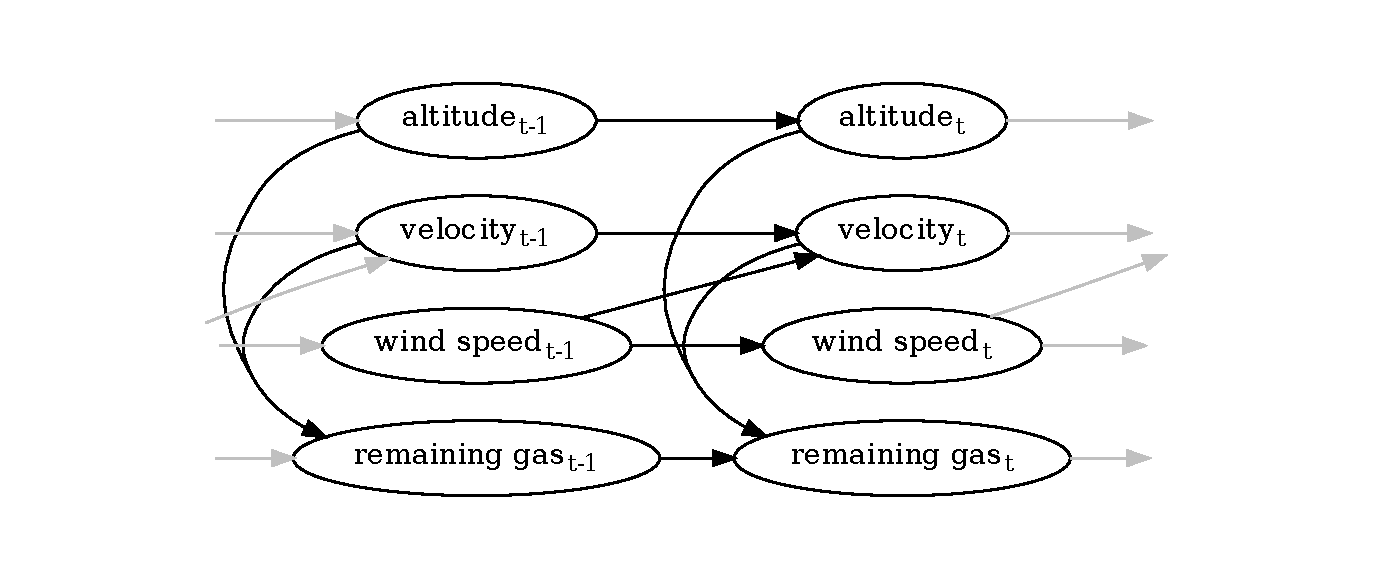
\includegraphics[width=1\textwidth]{dbn}
 	\caption{Visualization of a dynamic Bayesian network with four variables at time $t$.}
 	\label{fig:dbn}
\end{figure}

\section{Dynamic naive Bayesian classifier}

\subsection{Introduction}

Dynamic naive Bayesian classifier (DNBC) can be considered as an extension of hidden Markov model. The difference is in the number of observed variables. HMM defines only a single observed variable, whereas DNBC supports multiple observed variables.

DNBC is dynamic, because it classifies sequences with variables at every time $t$. It is called naive, because the output variables are assumed to be conditionally independent of each other. Figure \ref{fig:dnbc} demonstrates a walk through a model with 2 observed variables. 

\subsection{Description}

DNBC is defined by

\begin{figure}
	\centering
 	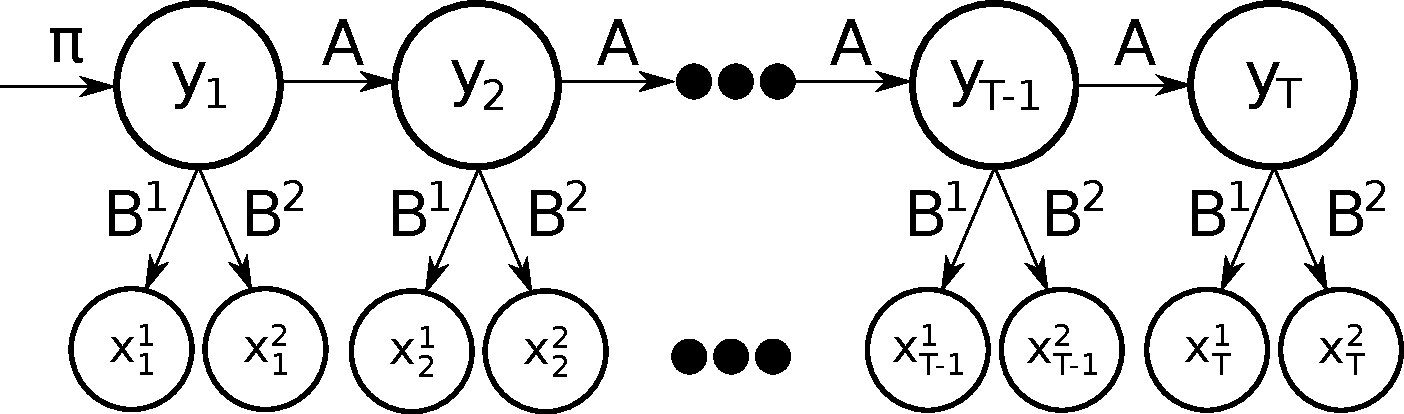
\includegraphics[width=0.7\textwidth]{dnbc}
 	\caption{Visualization of a dynamic naive Bayesian classifier with two observed variables. At each time point, there is a hidden state $y_t$ and two observed states: $x_t^1$ and $x_t^2$.}
 	\label{fig:dnbc}
\end{figure}

\begin{itemize}

\item{a number of observed variables $O$,}
\item a set of hidden states $S = \{S_1, S_2, \dots, S_N\}$,
\item{sets of observed symbols $X^j, j \in [1,O]$}
\item a transition matrix $A \in \textbf R^{N \times N}$,
\item observation probability functions $B^j = \{b_1^j(o), b_2^j(o), \dots, b_N^j(o)\}, j \in [1,O]$,
\item an initial probability vector $\pi \in \textbf R^N$.

\end{itemize}

The values of particular set of observed symbols $X^j$ can be either discrete or continuous. The values of $S$ are assumed to be discrete. The observation probability function $b_i^j(o)$ describes a probability $P(x^j_t=o|y_t=S_i)$, where $o \in X^j$. $b_i^j(o)$ is called an emission function.

Imagine a walk through DNBC graph. At time point $t$, there is a hidden state $y_t$ and $O$ observed symbols $x^j_t$, where $j \in [1,O]$. Value of each observed symbol conditionally depends on the value of the hidden state. The dependency is described by the emission function $b_i^j(o)$.

An important property of DNBC is that the observed variables are assumed to be independent of each other. Therefore, DNBC does not define any conditional dependency function between two observed variables.

If $t \neq 1$ and $T > 1$, there is a hidden state $y_t$ that conditionally depends on the value of previous hidden state $y_{t-1}$. The dependency is described by transition $a_{ij}$. If $t = 1$, there is a hidden state $y_1$ that conditionally depends on the initial transition $\pi_i$.

\subsection{Notation}
Let $\hat{x}_t$ be the observed variables at time $t$.
\begin{equation*}
\hat{x}_t = x_t^1, x_t^2, \dots, x_t^O.
\end{equation*}
It must hold that the number of observed variables at every time $t$ is the same.
Let $\textbf{x}_t$ be a sequence of observations up to time point t.
\begin{equation*}
\textbf{x}_t = \hat{x}_1, \hat{x}_2, \dots, \hat{x}_t.
\end{equation*}
For simplification, let's define $\textbf{x}$ to be all the observations of an input sequence.
\begin{equation*}
\textbf{x} = \textbf{x}_T.
\end{equation*}

\subsection{Operations}

Similarly to HMM, there are three common operations that can be performed on DNBC\textemdash learning, inference and scoring.

Learning is used to estimate the model parameters $\{\pi,A,B^1,B^2,\dots,B^O\} = \lambda$. It is desired to estimate the parameters such that $\prod_{j=1}^{M} P(\textbf x^j | \lambda )$ is maximized. Where $M \in \textbf N$ is a number of sequences to be learned. $\textbf x^j$ is a \emph{j}-th sequence of observed symbols. In other words, it is desired to maximize the product of probabilities that the given sequence of observed symbols was generated by the given model.

Inference returns the most likely sequence of hidden states, given sequences of observed symbols.

Given a sequence of observations $\textbf{x}$, what is the probability that it was generated by DNBC with parameters $\lambda$? Scoring answers this question.

\subsection{Learning}

The learning approach is similar to the one described in the case of HMM. The only difference is that there are multiple emission functions $b^j_i(o)$ where $j \in [1,O]$ and $O$ is the number of observed variables.

\subsection{Inference}

Viterbi algorithm can be applied in the similar way as in the case of HMM. It is extended to support multiple observed variables. Let's define $a_t(i)$ to be the maximum probability of sequence of hidden states and sequence of observations up to time point $t$:

\begin{equation} \label{eq:dnbc_viterbi_a}
a_t(i) = max_{y_1,y_2,\dots,y_{t-1}} P(y_1,y_2,\dots,y_{t-1},y_t = S_i,\textbf{x}_t| \lambda).
\end{equation}

\paragraph{Initialization}

At time point $t=1$, the probability of being at hidden state $S_i$ is equal to the initial probability of being at that state and probabilities of being at observed symbol $x_1^j$ given hidden state $S_i$. In other words:

\begin{equation*}
\alpha_1(i) = \pi_i \prod_{j=1}^O b^j_i(x^j_1).
\end{equation*}

\paragraph{Recursion}
Taking into account the structure of DNBC, the equation \ref{eq:dnbc_viterbi_a} can be rewritten recursively as

\begin{equation} \label{eq:dnbc_viterbi_a_rec}
\alpha_t(j) = [\max_i \alpha_{t-1}(i)a_{ij}] \prod_{k=1}^O b_j^k(x^k_t).
\end{equation}
Hidden state at particular time point $t$ is determined by

\begin{equation*}
s_t = S_{\argmax_i \alpha_{t}(i)}.
\end{equation*}

\paragraph{Complexity}

At each time point $t$ and hidden state index $j$, the equation \ref{eq:dnbc_viterbi_a_rec} loops through every hidden state index $i$ and every observed variable index $k$. There are $N$ hidden states and $O$ observed variables. In addition, the recursion continues for every time point $t$. There are $T$ time points. Thus, the overall time complexity is
$N(N+O) T$.

\subsection{Scoring}

Scoring is performed the same way as in case of HMM. That is, the score can be calculated as

\begin{equation*}
\sum_{i=1}^{N} \alpha_T(i).
\end{equation*}

\subsection{Example}

Consider a problem of weather prediction. Let's define a set of hidden states to be $S = \{S_1 = \text{sunny}, S_2 = \text{rainy}, S_3 = \text{cloudy} \}$. Let's consider the following observed variables: temperature, humidity and windiness. At every time $t$, the hidden state conditionally depends on the hidden state at time $t-1$. The three observed variables at time $t$ conditionally depend on the hidden state $t$. These variables can help in predicting the hidden state.

\subsection{Limitations}

The observed variables are assumed to be conditionally independent of each other. While this assumption enables the use of algorithms with relatively low time complexity and less data, it also limits the ability to describe more complicated relations among random variables. For example, the observed variables may be correlated in reality.

\chapter{Implementation} \label{ch:implementation}

There are no existing DNBC libraries written in Scala language. Although there exists a library for Bayesian networks \cite{bayesian-networks}, which is a super set of DNBC, it does not support computations on top of Apache Spark. Bayesian networks use different learning and inference algorithms than DNBC. Extending this library would thus be above scope of this thesis.

I have implemented a dynamic naive Bayesian classifier in Scala programming language that runs on top of Apache Spark. I named this software \textit{dnbc-scala}.

\section{Apache Spark}

Apache Spark is an engine for cluster-computing. It provides application programming interface (API) that developers can use to execute computations on multiple nodes\textemdash processors or machines in a cluster. Spark is also fault-tolerant, meaning that if a computation fails at given node, another node will take over.

When executing a program on top of Spark, it runs as a \textit{driver}. The driver passes execution of parallel operations such as \textit{map} or \textit{reduce} to Spark. These operations are then processed on multiple nodes in the cluster \cite{spark}.

Map and reduce are fundamental operations in functional programming. The map operation takes a set of input data and converts it into another set. For example, one can transform a set of strings into a set of their corresponding lengths. Reduce takes a set of input data and combines it together. For example, one can take a set of numbers and add them together.

The map operation assumes that the input data set can be independently converted into another set. This enables the operation to run in parallel. The reduce operation assumes that the input data can be combined in any order. Thus the operation can be also performed in parallel fashion.

Apache Spark is implemented in Scala programming language. The language combines functional and object-oriented programming. Scala code compiles into Java virtual machine (JVM) bytecode. This enables one to incorporate existing Java libraries into a Scala project.

\section{Project structure}

The project is divided into 5 modules:

\begin{itemize}

\item \textit{core}\textemdash main module containing DNBC interface, helper class for loading data set into required format and a class for measuring performance of DNBC on a data set,
\item \textit{core-test}\textemdash contains tests of $core$ module,
\item \textit{performance}\textemdash provides command line interface for generating a parametric data set and measuring DNBC performance on it,
\item \textit{preprocessing}\textemdash transforms a predefined data set into data sets with different parameters,
\item \textit{test-utils}\textemdash provides commonly used functions in tests or in performance measurement.

\end{itemize}

Figure \ref{fig:module-dependencies} provides overview of the project structure and module dependencies.

\begin{figure}
	\centering
 	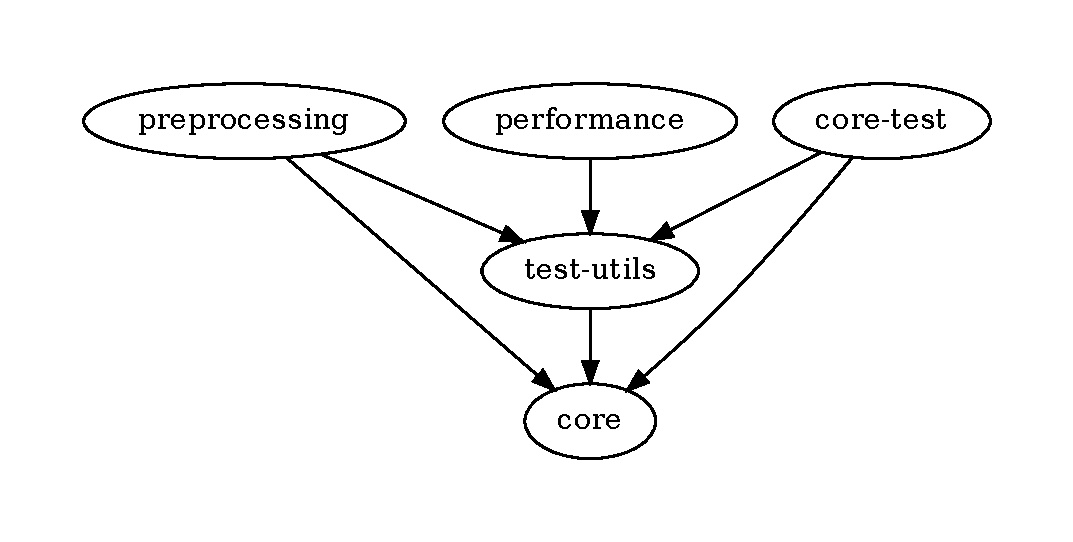
\includegraphics[width=0.7\textwidth]{module-dependencies}
 	\caption{Dependencies among modules in \textit{dnbc-scala} project.}
 	\label{fig:module-dependencies}
\end{figure}

\section{Usage}

\paragraph{DynamicNaiveBayesianClassifier object}

\textit{DynamicNaiveBayesianClassifier} object in \textit{core} module serves as a factory for already learned class \textit{DynamicNaiveBayesianClassifier}.

\begin{lstlisting}[style=myScalaStyle]
object DynamicNaiveBayesianClassifier {
  def mle(sc: SparkContext,
          sequences: Iterable[Seq[State]],
          continuousVariableHints: Option[List[Int]] = Option.empty)
          : DynamicNaiveBayesianClassifier
}
\end{lstlisting}

The function \textit{mle} returns a learned model. \textit{sequences} are sequences of \textit{States} used for learning. Optional argument \textit{continuousVariableHints} can be provided to set the number of components in Gaussian mixtures. The implementation does not try to estimate this number. If the parameter is not provided, the continuous variables are expected to be normally distributed.

The model parameters (\textit{Edges}) are learned in every sequence of states. After processing of all input sequences, learning is finalized by calling a function \textit{learnFinalize} on each edge. These functions are executed in parallel since their execution order is not important and they do not depend on each other.

\paragraph{Learned DNBC class}

This following class represents a DNBC model with known parameters.

\begin{lstlisting}[style=myScalaStyle]
class DynamicNaiveBayesianClassifier(
	initialEdge: LearnedDiscreteEdge,
	transitions: Map[String, LearnedDiscreteEdge],
	discreteEmissions: List[Map[String, LearnedDiscreteEdge]],
	continuousEmissions: List[Map[String, LearnedContinuousEdge]]) {
	def inferMostLikelyHiddenStates(observedStates: Seq[ObservedState]): List[String]
	def score(observedStates: Seq[ObservedState]): Double
}
\end{lstlisting}

The \textit{inferMostLikelyHiddenStates} function returns the most likely sequence of hidden states given a sequence of observed states. The function uses Viterbi algorithm. The following code is a function for Viterbi initialization.

\begin{lstlisting}[style=myScalaStyle]
  private def viterbiInitialize(observedStates: Seq[ObservedState]): Map[String,Double] = {
    var vcur = Map.empty[String,Double]
    for (hiddenState <- transitions.keys) {
      var emissionsSum = 0.0
      emissionsSum += discreteEmissions.zipWithIndex.map(z => Math.log(z._1(hiddenState)
      .probability(observedStates.head.DiscreteVariables(z._2)))).sum
      emissionsSum += continuousEmissions.zipWithIndex.map(z => Math.log(z._1(hiddenState)
      .probability(observedStates.head.ContinuousVariables(z._2)))).sum
      vcur += (hiddenState -> (emissionsSum + Math.log(initialEdge.probability(hiddenState))))
    }
    vcur
  }
\end{lstlisting}

The \textit{score} function returns a log-probability that given sequence of observed states was generated by the DNBC. It is internally using Viterbi algorithm to compute $\alpha_T(i)$.

The Viterbi algorithm is not implemented in parallel. The reason is that the algorithm proceeds by time points, and each time point depends on the previous one. At every time point, the parallelization is not worth it, since there is only a bunch of additions taking place.

\paragraph{State}

An observed state at given time point consists of observations of all the discrete and continuous variables. This is represented by \textit{ObservedState} class.

\begin{lstlisting}[style=myScalaStyle]
class ObservedState(discreteVariables: List[String], continuousVariables: List[Double]) {
  def DiscreteVariables: List[String] = discreteVariables
  def ContinuousVariables: List[Double] = continuousVariables
}
\end{lstlisting}

A state at given time point consists of a hidden state and an \textit{ObservedState}. Throughout the project, the hidden states are of \textit{String} type.

\begin{lstlisting}[style=myScalaStyle]
class State(hiddenState: String, observedState: ObservedState) {
  def HiddenState: String = hiddenState
  def ObservedState: ObservedState = observedState
}
\end{lstlisting}

\paragraph{Edge}

An edge represents a particular random variable, parameters of which are to be learned.

\begin{lstlisting}[style=myScalaStyle]
trait Edge[T] {
  def learn(occurrence: T): Unit
  def learnFinalize(): LearnedEdge[T]
}
\end{lstlisting}

The \textit{learn} function notifies an edge that \textit{occurrence} occurred. User calls \textit{learnFinalize} function to estimate the variable parameters based on previous occurrences.

There are two kinds of edges: \textit{DiscreteEdge} and \textit{ContinuousEdge}. As expected, \textit{DiscreteEdge} represents a discrete random variable, whereas \textit{ContinuousEdge} represents a continuous random variable.

To estimate the parameters of continuous random variables using MLE, I am using jMEF Java library. Previously I used Spark's MLlib library for estimating parameters of a Gaussian mixture model (GMM). The problem with this is approach was that it can only estimate the parameters by making a computation across multiple nodes in a cluster. This is not a desired behavior since there are many estimations of small data that should run in parallel instead. Therefore, I ended up using jMEF library which estimates the parameters in sequential fashion.

\paragraph{LearnedEdge}

A \textit{LearnedEdge} represents a random variable which parameters have been already estimated. The \textit{probability} function returns a probability that a state occurs.

\begin{lstlisting}[style=myScalaStyle]
trait LearnedEdge[T] {
  def probability(state: T): Double
}
\end{lstlisting}

\paragraph{RandomEdge}

A \textit{RandomEdge} generates random value given random variable parameters. This is useful for performance measurement, where data sets are randomly generated.

\begin{lstlisting}[style=myScalaStyle]
trait RandomEdge[T] {
  def next(): T
}
\end{lstlisting}

\section{Underflow}

Since the Viterbi algorithm is computing products of probabilities, the resulting value gets small in few iterations. To avoid underflow, one can compute a log-probability instead, using the following trick:

\begin{equation*}
\log(abc) = \log(a)+\log(b)+\log(c).
\end{equation*}
Now instead of multiplying tiny numbers together, one can use addition.

\section{Data set generation}

The \textit{test-utils} module contains a function \textit{generatePerformanceDataSet}. This generates a random data set, given parameters. The data set can be used for measuring learning and testing time. The supported parameters are:

\begin{enumerate}
	\item the length of sequences,
	\item the number of training sequences,
	\item the number of testing sequences,
	\item the number of hidden states,
	\item the number of discrete observed variables,
	\item the number of continuous observed variables,
	\item the maximum number of components per mixture,
	\item the number of transitions per hidden state.
\end{enumerate}

The initial edge probabilities are generated by choosing random number from a Gaussian distribution. The numbers are then normalized to ensure their sum is equal to one. Every hidden state's transition destination is chosen randomly from an uniform distribution. The probabilities of transitions are then set the same way as in case of initial edge. Same approach is used for discrete emissions.

For continuous emissions, the parameters of GMM are chosen randomly in uniform fashion in range of these parameters:

\begin{equation*}
\mu \in [-10,10],
\sigma^2 \in [1,4].
\end{equation*}
The weights in a \textit{RandomContinuousEdge} are all equal.

\section{Source code}
The implementation is available on GitHub \cite{dnbc-scala} or via the provided USB flash drive as part of this thesis.

\chapter{Experiments}

\section{Unit tests}

I am using a Toy Robot data set \cite{robot-maze} as a base data set for unit tests. Imagine a robot wandering through a maze. There are 12 hidden states. Every hidden state is a 2D coordinate. Every hidden state has an associated color. The color is a discrete observed variable consisting of 4 states: red, green, blue and yellow. The initial state is chosen randomly. The data set contains of 200 training sequences and 200 test sequences. Every sequence consists of 200 time points. 10\% of the data set observed states at time points are chosen at random. This depicts robot's occasional failure to detect correct color.

\begin{figure}
	\centering
 	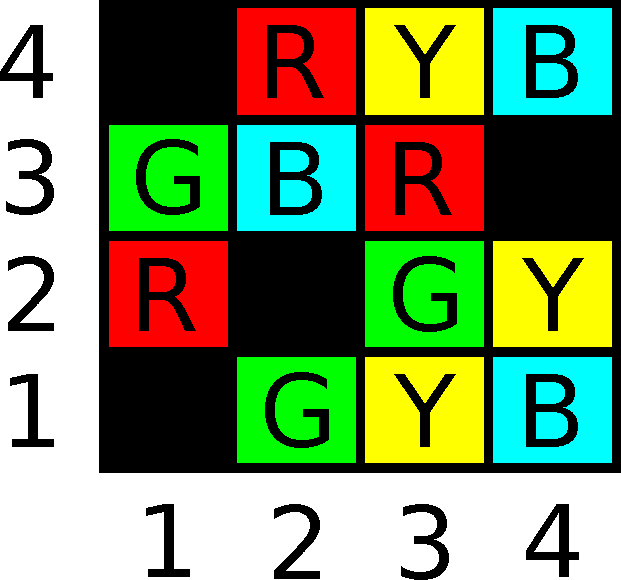
\includegraphics[width=0.4\textwidth]{robot_maze}
 	\caption{Visualization of a Toy Robot data set \cite{robot-maze}.}
 	\label{fig:robot_maze}
\end{figure}

\paragraph{Measurement}
For every data set in unit tests, an average success rate (ASR) is measured. This average is the average percentage of hidden states inferred correctly in the testing phase.

\paragraph{Discrete variable}
ASR on the Toy Robot data set is 65\%.

\paragraph{Continuous variable}
The Toy Robot data set is transformed to have a single continuous observed variable instead. Every color (discrete random variable) is replaced by temperature. The idea is that the 4 colors have different temperature distributions if sun is shedding light on the maze. ASR of this data set is 42\%.

\paragraph{Discrete and continuous variable}
A discrete observed variable is added to the continuous variable data set. This variable describes the quadrant of given 2D coordinate. It is assumed that these two variables are independent. ASR of this data set is 76\%.

\paragraph{Gaussian mixture}
A data set with single continuous observed variable is generated. Hidden states can take on two values: true and false. If the hidden state is true, observed state is generated from a Gaussian distribution. If the hidden state is false, observed state is generated from a Gaussian mixture distribution. Point of this test is to check that providing a variable hint describing the number of mixture components improves the ASR. ASR with correctly set variable hint is 3\% higher compared to a case where no hint is set.

\paragraph{Scoring}
A score is computed for a sequence of observed states that comes from a data set a DNBC was trained on. Another score is computed for a sequence of observed states that was generated randomly. Since the score is a log-probability, the values are negative. The following holds:

\begin{lstlisting}[language=Scala]
assert ( scoreReal*1.5 > scoreRandom ).
\end{lstlisting}

\section{Performance}

In this section, I focus on learning and testing time given a generated parametric data set. The measurements were made on a machine specified in table \ref{tab:machine-specification}. Every job was assigned 15 GB RAM and 10 GB disk space.

\begin{table}
\centering
\begin{tabular}{|c|c|}
	\hline
	CPU & 2x 8-core Intel Xeon E5-2650 v2 2.6 GHz \\
	RAM & 96 GB \\
	disk & 2x500 GB HDD WD Velociraptor 10k SATA \\
	\hline
\end{tabular}
\caption{Machine specification \cite{machine-specification}}
\label{tab:machine-specification}
\end{table}

The base parameters used for data set generations and performance measurement are described in table \ref{tab:base-parameters}.

\begin{table}
\centering
\begin{tabular}{|c|c|}
	\hline
	number of processors & 2 \\
	length of sequences & 200 \\
	number of training sequences & 1000 \\
	number of testing sequences & 200 \\
	number of hidden states & 10 \\
	number of discrete observed variables & 5 \\
	number of continuous observed variables & 5 \\
	max number of components per mixture & 3 \\
	transitions per hidden state & 5 \\
	\hline
\end{tabular}
\caption{Base data set generation and evaluation parameters.}
\label{tab:base-parameters}
\end{table}

\paragraph{Local scalability}

Goal of this measurement is to see how well the software scales as we increase number of processors. Figure \ref{fig:parallel_learning_time} shows results of this measurement. Every configuration was measured 4 times to enable better understanding of the data. The data sets had 30 discrete and 30 continuous observed variables.

\begin{figure}
	\centering
 	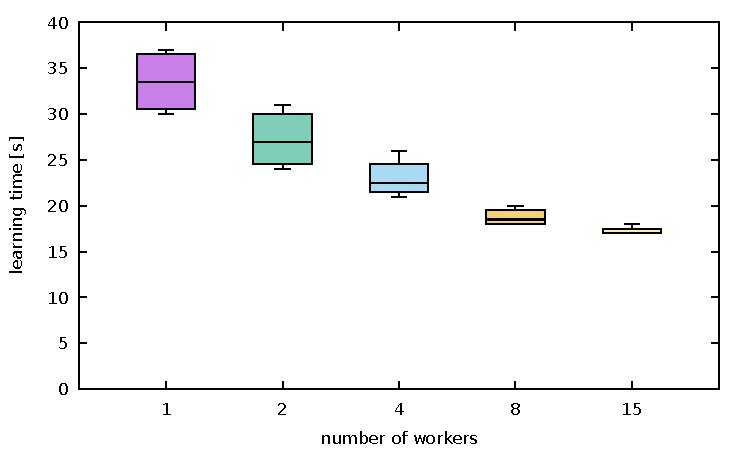
\includegraphics[width=0.7\textwidth]{parallel_learning_time}
 	\caption{Learning time per number of workers.}
 	\label{fig:parallel_learning_time}
\end{figure}

As it can be seen, the software does not scale particularly well. In fact, the majority of time is spent reading the data set data. This is not a parallel operation. Reading data is the bottleneck.

To focus on scalability of learning itself, figure \ref{fig:parallel_continuous_emissions_learning_time} shows learning time of all continuous emissions, without the data loading. As it can be seen, this segment scales relatively well.

\begin{figure}
	\centering
 	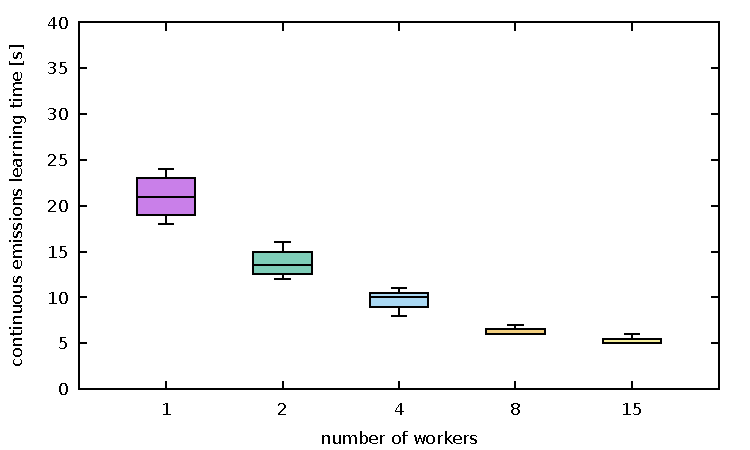
\includegraphics[width=0.7\textwidth]{parallel_continuous_emissions_learning_time}
 	\caption{Continuous emissions learning time per number of workers.}
 	\label{fig:parallel_continuous_emissions_learning_time}
\end{figure}

\paragraph{Cluster scalability}

In this experiment, I set up 8 independent worker nodes in a cluster. Every worker is assigned 15 GB RAM and 10 GB disk space. The goal is to measure scalability as the number of processors per node increases. The data sets had 100 discrete and 100 continuous observed variables. As it can be seen on figure \ref{fig:cluster_continuous_learning_time}, the continuous emissions learning time is about 45\% lower when using $8 \times 4$ processors in comparison to using 8 processors.

\begin{figure}
	\centering
 	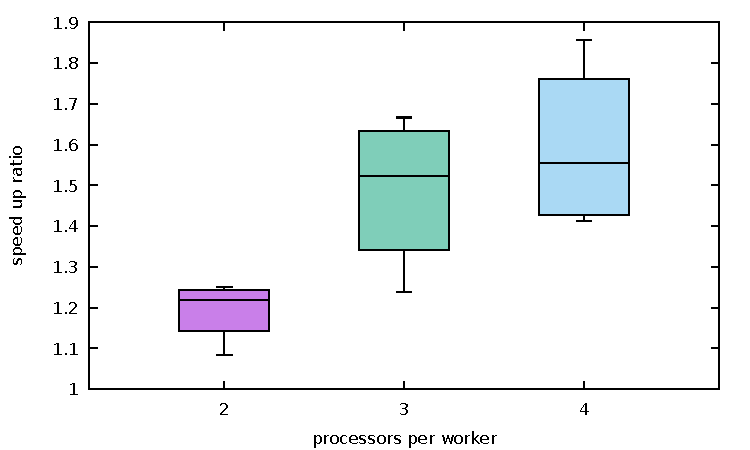
\includegraphics[width=0.7\textwidth]{cluster_continuous_learning_time}
 	\caption{Continuous emissions learning time per number of processors per worker.}
 	\label{fig:cluster_continuous_learning_time}
\end{figure}

\paragraph{Training sequences}

Figure \ref{fig:learning_set_learning_time} shows approximately linear complexity as number of training sequences increases.

\begin{figure}
	\centering
 	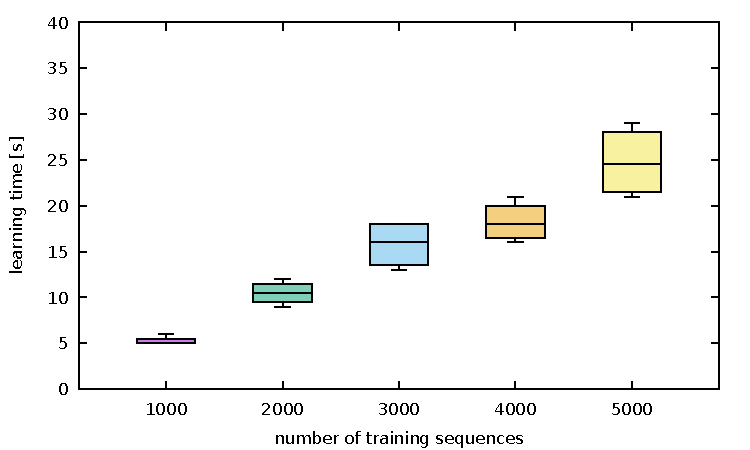
\includegraphics[width=0.7\textwidth]{learning_set_learning_time}
 	\caption{Learning time per number of training sequences.}
 	\label{fig:learning_set_learning_time}
\end{figure}

\paragraph{Hidden states}

Interestingly, as we increase the number of hidden states, the learning time does not change. Testing time increases super-linearly. This can be see in figure \ref{fig:hidden_states_learning_testing_time}.

\begin{figure}
	\centering
 	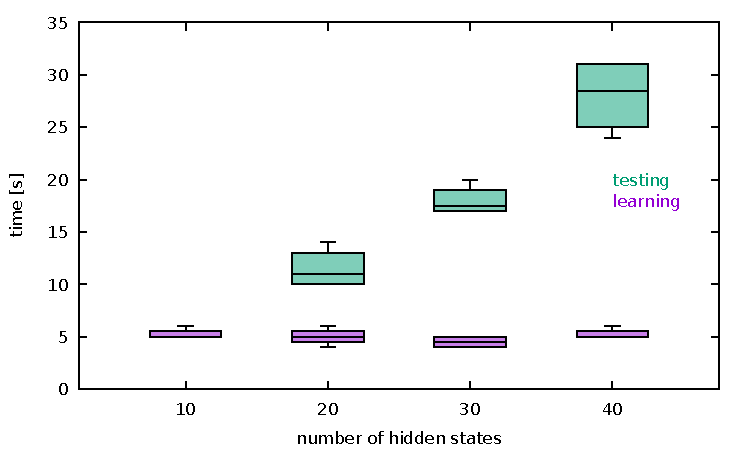
\includegraphics[width=0.7\textwidth]{hidden_states_learning_testing_time}
 	\caption{Learning and testing times per number of hidden states.}
 	\label{fig:hidden_states_learning_testing_time}
\end{figure}

\paragraph{Discrete variables}

As the number of observed discrete variables increases, both learning and testing times increase approximately linearly. See figures \ref{fig:discrete_variables_learning_time} and \ref{fig:discrete_variables_testing_time}.

\paragraph{Continuous variables}

Similar phenomenon can be seen when the number of observed continuous variables increases. The plot looks very similar to the one where number of discrete variables is being increased.

\begin{figure}
	\centering
 	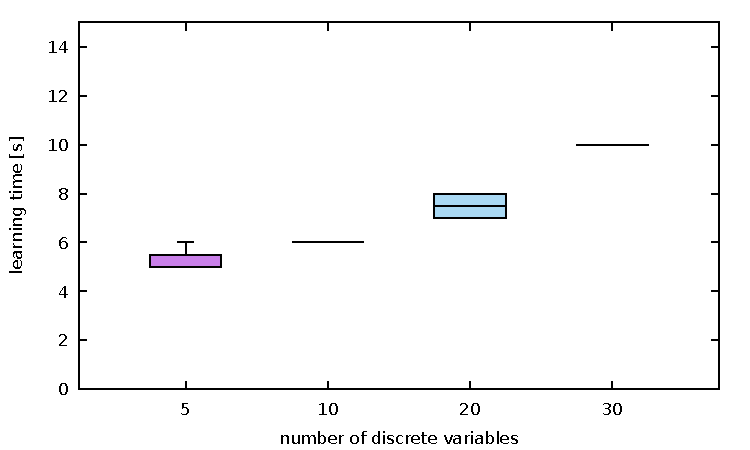
\includegraphics[width=0.7\textwidth]{discrete_variables_learning_time}
 	\caption{Learning time per number of observed discrete variables.}
 	\label{fig:discrete_variables_learning_time}
\end{figure}

\begin{figure}
	\centering
 	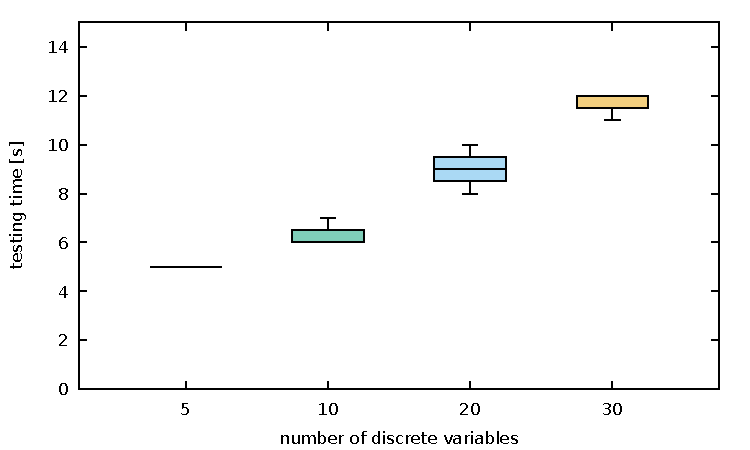
\includegraphics[width=0.7\textwidth]{discrete_variables_testing_time}
 	\caption{Testing time per number of observed discrete variables.}
 	\label{fig:discrete_variables_testing_time}
\end{figure}

\begin{conclusion}
I have described the theory behind dynamic naive Bayesian classifier (DNBC) and other models it is based on. Since no known viable implementation currently exists in Scala, I have decided to implement DNBC by myself. I have demonstrated correctness of my implementation through unit tests. Furthermore, the software shows promising results in terms of speed up when used in a system with multiple processors. Future improvement could be to implement an alternative learning algorithm: Baum-Welch training, and compare it to existing maximum likelihood estimation (MLE) based learning.
\end{conclusion}

\bibliographystyle{csn690}
\bibliography{bibliography}

\appendix

\chapter{List of abbreviations}
% \printglossaries
\begin{description}
	\item[ASR] average success rate
	\item[API] application programming interface
	\item[CPT] conditional probability table
	\item[DAG] dynamic acyclic graph
	\item[DNBC] dynamic naive Bayesian classifier
	\item[EM] expectation-maximization
	\item[GMM] Gaussian mixture model
	\item[HMM] hidden Markov model
	\item[i.i.d.] independent, identically distributed
	\item[JVM] Java virtual machine
	\item[PDF] probability density function
	\item[MC] Markov chain
\end{description}

% % % % % % % % % % % % % % % % % % % % % % % % % % % % 
% % Tuto kapitolu z výsledné práce ODSTRAŇTE.
% % % % % % % % % % % % % % % % % % % % % % % % % % % % 
% 
% \chapter{Návod k~použití této šablony}
% 
% Tento dokument slouží jako základ pro napsání závěrečné práce na Fakultě informačních technologií ČVUT v~Praze.
% 
% \section{Výběr základu}
% 
% Vyberte si šablonu podle druhu práce (bakalářská, diplomová), jazyka (čeština, angličtina) a kódování (ASCII, \mbox{UTF-8}, \mbox{ISO-8859-2} neboli latin2 a nebo \mbox{Windows-1250}). 
% 
% V~české variantě naleznete šablony v~souborech pojmenovaných ve formátu práce\_kódování.tex. Typ může být:
% \begin{description}
% 	\item[BP] bakalářská práce,
% 	\item[DP] diplomová (magisterská) práce.
% \end{description}
% Kódování, ve kterém chcete psát, může být:
% \begin{description}
% 	\item[UTF-8] kódování Unicode,
% 	\item[ISO-8859-2] latin2,
% 	\item[Windows-1250] znaková sada 1250 Windows.
% \end{description}
% V~případě nejistoty ohledně kódování doporučujeme následující postup:
% \begin{enumerate}
% 	\item Otevřete šablony pro kódování UTF-8 v~editoru prostého textu, který chcete pro psaní práce použít -- pokud můžete texty s~diakritikou normálně přečíst, použijte tuto šablonu.
% 	\item V~opačném případě postupujte dále podle toho, jaký operační systém používáte:
% 	\begin{itemize}
% 		\item v~případě Windows použijte šablonu pro kódování \mbox{Windows-1250},
% 		\item jinak zkuste použít šablonu pro kódování \mbox{ISO-8859-2}.
% 	\end{itemize}
% \end{enumerate}
% 
% 
% V~anglické variantě jsou šablony pojmenované podle typu práce, možnosti jsou:
% \begin{description}
% 	\item[bachelors] bakalářská práce,
% 	\item[masters] diplomová (magisterská) práce.
% \end{description}
% 
% \section{Použití šablony}
% 
% Šablona je určena pro zpracování systémem \LaTeXe{}. Text je možné psát v~textovém editoru jako prostý text, lze však také využít specializovaný editor pro \LaTeX{}, např. Kile.
% 
% Pro získání tisknutelného výstupu z~takto vytvořeného souboru použijte příkaz \verb|pdflatex|, kterému předáte cestu k~souboru jako parametr. Vhodný editor pro \LaTeX{} toto udělá za Vás. \verb|pdfcslatex| ani \verb|cslatex| \emph{nebudou} s~těmito šablonami fungovat.
% 
% Více informací o~použití systému \LaTeX{} najdete např. v~\cite{wikilatex}.
% 
% \subsection{Typografie}
% 
% Při psaní dodržujte typografické konvence zvoleného jazyka. České \uv{uvozovky} zapisujte použitím příkazu \verb|\uv|, kterému v~parametru předáte text, jenž má být v~uvozovkách. Anglické otevírací uvozovky se v~\LaTeX{}u zadávají jako dva zpětné apostrofy, uzavírací uvozovky jako dva apostrofy. Často chybně uváděný symbol "{} (palce) nemá s~uvozovkami nic společného.
% 
% Dále je třeba zabránit zalomení řádky mezi některými slovy, v~češtině např. za jednopísmennými předložkami a spojkami (vyjma \uv{a}). To docílíte vložením pružné nezalomitelné mezery -- znakem \texttt{\textasciitilde}. V~tomto případě to není třeba dělat ručně, lze použít program \verb|vlna|.
% 
% Více o~typografii viz \cite{kobltypo}.
% 
% \subsection{Obrázky}
% 
% Pro umožnění vkládání obrázků je vhodné použít balíček \verb|graphicx|, samotné vložení se provede příkazem \verb|\includegraphics|. Takto je možné vkládat obrázky ve formátu PDF, PNG a JPEG jestliže používáte pdf\LaTeX{} nebo ve formátu EPS jestliže používáte \LaTeX{}. Doporučujeme preferovat vektorové obrázky před rastrovými (vyjma fotografií).
% 
% \subsubsection{Získání vhodného formátu}
% 
% Pro získání vektorových formátů PDF nebo EPS z~jiných lze použít některý z~vektorových grafických editorů. Pro převod rastrového obrázku na vektorový lze použít rasterizaci, kterou mnohé editory zvládají (např. Inkscape). Pro konverze lze použít též nástroje pro dávkové zpracování běžně dodávané s~\LaTeX{}em, např. \verb|epstopdf|.
% 
% \subsubsection{Plovoucí prostředí}
% 
% Příkazem \verb|\includegraphics| lze obrázky vkládat přímo, doporučujeme však použít plovoucí prostředí, konkrétně \verb|figure|. Například obrázek \ref{fig:float} byl vložen tímto způsobem. Vůbec přitom nevadí, když je obrázek umístěn jinde, než bylo původně zamýšleno -- je tomu tak hlavně kvůli dodržení typografických konvencí. Namísto vynucování konkrétní pozice obrázku doporučujeme používat odkazování z~textu (dvojice příkazů \verb|\label| a \verb|\ref|).
% 
% \begin{figure}\centering
% 	
\includegraphics[width=0.5\textwidth, angle=30]{cvut-logo-bw}
% 	\caption[Příklad obrázku]{Ukázkový obrázek v~plovoucím prostředí}\label{fig:float}
% \end{figure}
% 
% \subsubsection{Verze obrázků}
% 
% % Gnuplot BW i barevně
% Může se hodit mít více verzí stejného obrázku, např. pro barevný či černobílý tisk a nebo pro prezentaci. S~pomocí některých nástrojů na generování grafiky je to snadné.
% 
% Máte-li například graf vytvořený v programu Gnuplot, můžete jeho černobílou variantu (viz obr. \ref{fig:gnuplot-bw}) vytvořit parametrem \verb|monochrome dashed| příkazu \verb|set term|. Barevnou variantu (viz obr. \ref{fig:gnuplot-col}) vhodnou na prezentace lze vytvořit parametrem \verb|colour solid|.
% 
% \begin{figure}\centering
% 	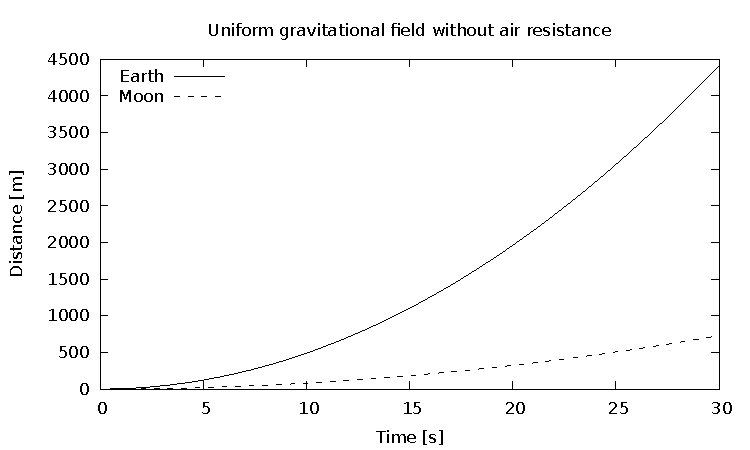
\includegraphics{gnuplot-bw}
% 	\caption{Černobílá varianta obrázku generovaného programem Gnuplot}\label{fig:gnuplot-bw}
% \end{figure}
% 
% \begin{figure}\centering
% 	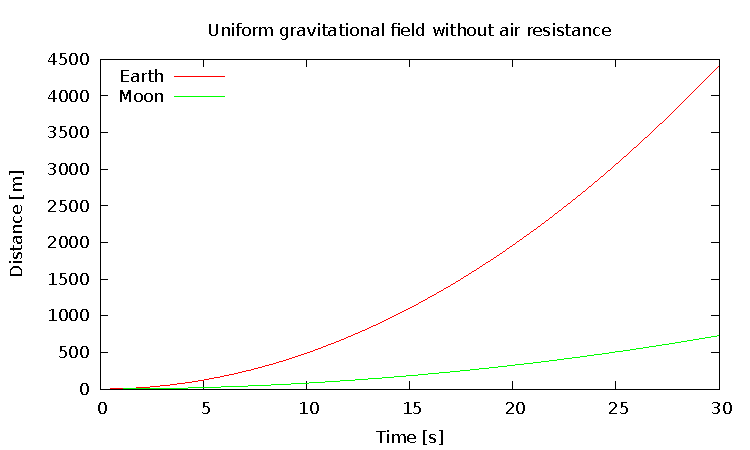
\includegraphics{gnuplot-col}
% 	\caption{Barevná varianta obrázku generovaného programem Gnuplot}\label{fig:gnuplot-col}
% \end{figure}
% 
% 
% \subsection{Tabulky}
% 
% Tabulky lze zadávat různě, např. v~prostředí \verb|tabular|, avšak pro jejich vkládání platí to samé, co pro obrázky -- použijte plovoucí prostředí, v~tomto případě \verb|table|. Například tabulka \ref{tab:matematika} byla vložena tímto způsobem.
% 
% \begin{table}\centering
% 	\caption[Příklad tabulky]{Zadávání matematiky}\label{tab:matematika}
% 	\begin{tabular}{|l|l|c|c|}\hline
% 		Typ		& Prostředí		& \LaTeX{}ovská zkratka	& \TeX{}ovská zkratka	\tabularnewline \hline \hline
% 		Text		& \verb|math|		& \verb|\(...\)|	& \verb|$...$|		\tabularnewline \hline
% 		Displayed	& \verb|displaymath|	& \verb|\[...\]|	& \verb|$$...$$|	\tabularnewline \hline
% 	\end{tabular}
% \end{table}
% 
% % % % % % % % % % % % % % % % % % % % % % % % % % % % 

\chapter{Obsah přiloženého CD}

%upravte podle skutecnosti

\begin{figure}
	\dirtree{%
		.1 readme.txt\DTcomment{stručný popis obsahu CD}.
		.1 exe\DTcomment{adresář se spustitelnou formou implementace}.
		.1 src.
		.2 impl\DTcomment{zdrojové kódy implementace}.
		.2 thesis\DTcomment{zdrojová forma práce ve formátu \LaTeX{}}.
		.1 text\DTcomment{text práce}.
		.2 thesis.pdf\DTcomment{text práce ve formátu PDF}.
		.2 thesis.ps\DTcomment{text práce ve formátu PS}.
	}
\end{figure}

\end{document}
